% figures/plan-classification.tex
% SwagePlan host classification: segment lengths bucketed into warp,
% cta, and split, producing four task lists.
\documentclass[tikz,border=10pt]{standalone}
% figures/common-preamble.tex
% Shared setup for the TikZ documentation figures. Colors mirror the
% palette in scripts/render_docs_diagrams.py so both atlases match.
\usepackage[T1]{fontenc}
\usepackage{lmodern}
\usepackage{tikz}
\usepackage{pgfplots}
\pgfplotsset{compat=1.18}
\usetikzlibrary{arrows.meta}
\usetikzlibrary{backgrounds}
\usetikzlibrary{calc}
\usetikzlibrary{decorations.pathreplacing}
\usetikzlibrary{fit}
\usetikzlibrary{positioning}

\definecolor{swcanvas}{HTML}{FFFDF8}
\definecolor{swpanel}{HTML}{F5F3ED}
\definecolor{swink}{HTML}{17212B}
\definecolor{swmuted}{HTML}{4B5563}
\definecolor{swline}{HTML}{59636E}
\definecolor{swblue}{HTML}{00689D}
\definecolor{swbluefill}{HTML}{DCEFFD}
\definecolor{swpurple}{HTML}{8E4775}
\definecolor{swpurplefill}{HTML}{F7E2EF}
\definecolor{sworange}{HTML}{A94500}
\definecolor{sworangefill}{HTML}{FCE5DC}
\definecolor{swgreen}{HTML}{00664B}
\definecolor{swgreenfill}{HTML}{DDF4EB}
\definecolor{swgrayfill}{HTML}{EEF0F2}

\pagecolor{swcanvas}
\AtBeginDocument{\color{swink}}

\tikzset{
  swcell/.style={
    draw, minimum width=0.46cm, minimum height=0.46cm, inner sep=0pt,
    line width=0.7pt, rounded corners=1pt},
  swbox/.style={
    draw=swline, fill=swpanel, rounded corners=6pt, line width=0.9pt},
  swarrow/.style={-{Stealth[length=6pt]}, draw=swline, line width=1pt},
  swtag/.style={
    draw, rounded corners=8pt, line width=0.9pt,
    font=\bfseries\scriptsize, inner xsep=8pt, inner ysep=4pt},
  swtitle/.style={anchor=west, font=\Large\bfseries, text=swink},
  swsubtitle/.style={anchor=west, font=\small, text=swmuted},
  swcode/.style={font=\small\ttfamily, text=swink},
  every picture/.style={line cap=round},
}

\begin{document}
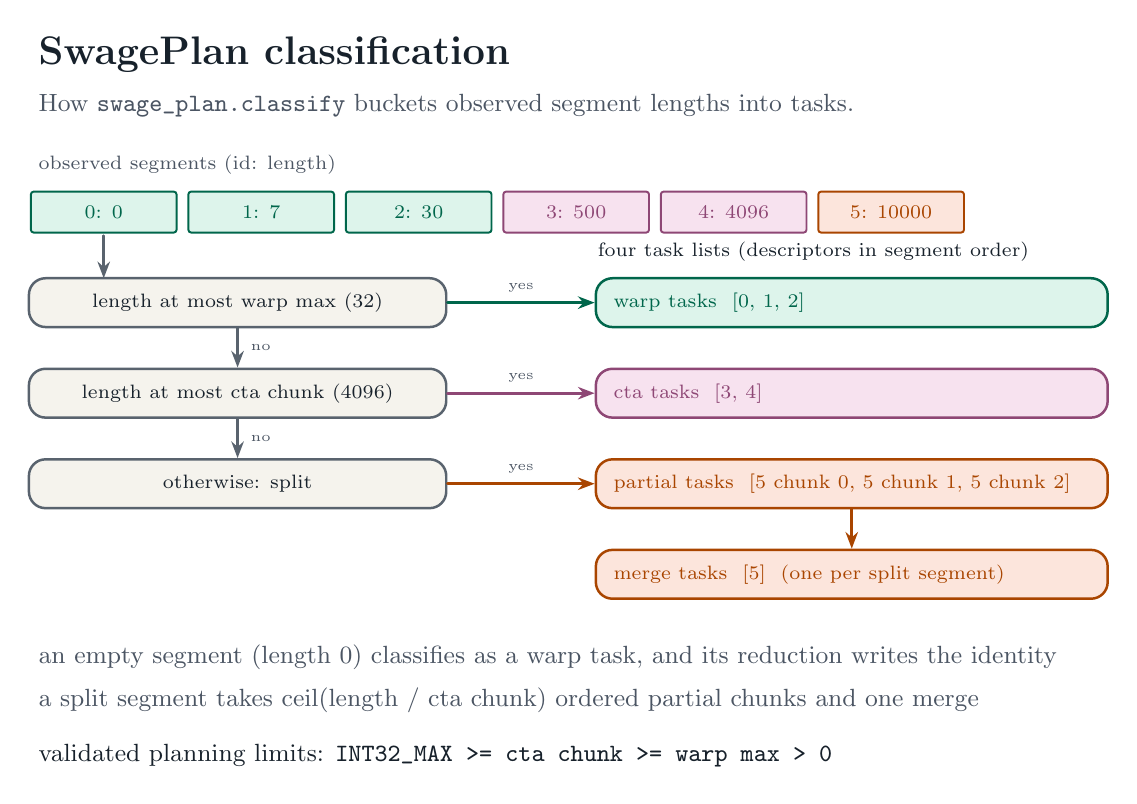
\begin{tikzpicture}[x=1cm, y=1cm]

% Header.
\node[swtitle] at (0, 1.15) {SwagePlan classification};
\node[swsubtitle] at (0, 0.5)
  {How {\ttfamily\detokenize{swage_plan.classify}} buckets observed
   segment lengths into tasks.};

% Observed segments with their lengths.
\node[anchor=west, font=\scriptsize, text=swmuted] at (0, -0.25)
  {observed segments (id: length)};
\foreach \i/\len/\col/\fil in {%
    0/0/swgreen/swgreenfill,
    1/7/swgreen/swgreenfill,
    2/30/swgreen/swgreenfill,
    3/500/swpurple/swpurplefill,
    4/4096/swpurple/swpurplefill,
    5/10000/sworange/sworangefill} {
  \node[swcell, minimum width=1.85cm, minimum height=0.52cm,
        fill=\fil, draw=\col] (seg\i) at (0.95 + \i * 2.0, -0.85) {};
  \node[font=\scriptsize, text=\col] at (0.95 + \i * 2.0, -0.85)
    {\i: \len};
}

% Decision ladder, one rule per row.
\draw[swarrow] (0.95, -1.15) -- (0.95, -1.69);
\foreach \row/\cond in {%
    0/{length at most warp max (32)},
    1/{length at most cta chunk (4096)},
    2/{otherwise: split}} {
  \node[swbox, minimum width=5.3cm, minimum height=0.62cm]
    (cond\row) at (2.65, {-2.0 - \row * 1.15}) {};
  \node[font=\scriptsize, text=swink]
    at (2.65, {-2.0 - \row * 1.15}) {\cond};
}
\foreach \row in {0, 1} {
  \pgfmathtruncatemacro{\next}{\row + 1}
  \draw[swarrow] (cond\row.south) -- (cond\next.north)
    node[midway, right=1pt, font=\tiny, text=swmuted] {no};
}

% The four task lists the classifier materializes.
\node[anchor=west, font=\scriptsize, text=swink] at (7.1, -1.35)
  {four task lists (descriptors in segment order)};
\foreach \row/\name/\body/\col/\fil in {%
    0/{warp tasks}/{[0, 1, 2]}/swgreen/swgreenfill,
    1/{cta tasks}/{[3, 4]}/swpurple/swpurplefill,
    2/{partial tasks}/{[5 chunk 0, 5 chunk 1, 5 chunk 2]}/%
      sworange/sworangefill} {
  \node[swbox, draw=\col, fill=\fil, minimum width=6.5cm,
        minimum height=0.62cm] (bucket\row)
    at (10.45, {-2.0 - \row * 1.15}) {};
  \node[anchor=west, font=\scriptsize, text=\col]
    at (7.3, {-2.0 - \row * 1.15}) {\name~~\body};
  \draw[swarrow, draw=\col] (cond\row.east) -- (bucket\row.west)
    node[midway, above=0pt, font=\tiny, text=swmuted] {yes};
}
\node[swbox, draw=sworange, fill=sworangefill, minimum width=6.5cm,
      minimum height=0.62cm] (merge) at (10.45, -5.45) {};
\node[anchor=west, font=\scriptsize, text=sworange] at (7.3, -5.45)
  {merge tasks~~[5]~~(one per split segment)};
\draw[swarrow, draw=sworange] (bucket2.south) -- (merge.north);

% Reading notes and the validated planning-limit invariant.
\node[anchor=west, font=\small, text=swmuted] at (0, -6.5)
  {an empty segment (length 0) classifies as a warp task, and its
   reduction writes the identity};
\node[anchor=west, font=\small, text=swmuted] at (0, -7.05)
  {a split segment takes ceil(length / cta chunk) ordered partial
   chunks and one merge};
\node[anchor=west, font=\small, text=swink] at (0, -7.75)
  {validated planning limits:
   {\ttfamily\detokenize{INT32_MAX >= cta chunk >= warp max > 0}}};

\end{tikzpicture}
\end{document}
